\documentclass[aspectratio=169,10pt]{beamer}
\usetheme{Madrid}
\usecolortheme{seahorse}
\setbeamertemplate{navigation symbols}{}
\usepackage{booktabs}
\usepackage{siunitx}
\usepackage{graphicx}
\usepackage{amsmath}
\usepackage{amssymb}
\usepackage{xcolor}
\usepackage{colortbl}
\graphicspath{{figures/}}

\definecolor{boxblue}{HTML}{2980b9}
\definecolor{boxgreen}{HTML}{16a085}
\definecolor{boxred}{HTML}{c0392b}
\definecolor{boxpurple}{HTML}{8e44ad}
\definecolor{boxgrey}{HTML}{ecf0f1}

% Helper command for coloured info boxes (tcolorbox substitute)
\newcommand{\infobox}[3]{%
  % #1 = frame colour, #2 = title text, #3 = body content
  \begin{beamercolorbox}[wd=\linewidth,sep=4pt,rounded=true,
        shadow=false,colsep*=0pt]{}%
    \color{#1}\textbf{#2}\\[2pt]
    \color{black}\footnotesize #3%
  \end{beamercolorbox}%
}

\title{Joint Placement-Policy Optimisation for Charging Stations in RMFS}
\subtitle{A Constrained RSM and Taguchi Robustness Approach}
\author{Salsa Zahrani}
\institute{Engineering Management \\ Institut Teknologi Bandung}
\date{}

\begin{document}

\maketitle

% ─────────────────────────────────────────────────────────────────────
\begin{frame}{Problem Statement --- The Single-Axis Trap}
  \begin{columns}[T]
    \column{0.5\textwidth}
    \footnotesize
    \textbf{What an RMFS warehouse needs to decide:}
    \begin{itemize}
      \item \textbf{Where} to install charging stations \\ (a CapEx commitment).
      \item \textbf{When} a robot should go charge, and how full to charge \\ (an OpEx parameter).
    \end{itemize}

    \vspace{0.4em}
    \textbf{The literature treats them separately:}
    \begin{itemize}
      \item Placement studies fix the policy and ask ``where?''
      \item Policy studies fix the placement and ask ``when?''
    \end{itemize}

    \column{0.5\textwidth}
    \footnotesize
    \textbf{The hypothesis:}
    \begin{itemize}
      \item Placement and policy \emph{interact}.
      \item Joint optimisation reveals failure modes invisible to either axis alone --- e.g., \textbf{deadlock manifolds} that emerge from the combination of policy thresholds and charger geometry.
    \end{itemize}

    \vspace{0.4em}
    \textbf{Our research question:}
    Given a joint design space (placement $\times$ policy $\times$ budget), what is the operationally robust optimum, and what statistical machinery surfaces it?
  \end{columns}
\end{frame}

% ─────────────────────────────────────────────────────────────────────
\begin{frame}{Research Contributions}
  \footnotesize
  \textbf{Methodological:}
  \begin{itemize}
    \item Treatment of discovered deadlock zones as \emph{infeasibility constraints} rather than missing data --- preserves statistical defensibility, turns failures into research findings.
    \item Single-seed deterministic DoE protocol with formal-test-free residual diagnostics for simulation environments.
  \end{itemize}

  \vspace{0.3em}
  \textbf{Empirical:}
  \begin{itemize}
    \item Placement quality dominates charger-budget by $\sim 30\times$ on long-horizon replenish ratio.
    \item Constrained-RSM optimum is also the Taguchi-robust optimum (rare in practice; both axes pointing the same direction).
    \item Initial battery state at shift start is the \emph{dominant} noise lever, not demand swing or fleet attrition.
  \end{itemize}

  \vspace{0.3em}
  \textbf{Managerial (decision-grade output):}
  \begin{itemize}
    \item A CapEx-OpEx-Procedural triple (placement, policy, operating practice) directly deployable in industry, each tier traceable to a specific experimental phase and defended by its own statistical artefact.
  \end{itemize}
\end{frame}

% ─────────────────────────────────────────────────────────────────────
\begin{frame}{Methodology --- Phased DoE Framework}
  \begin{columns}[T]
    \column{0.55\textwidth}
    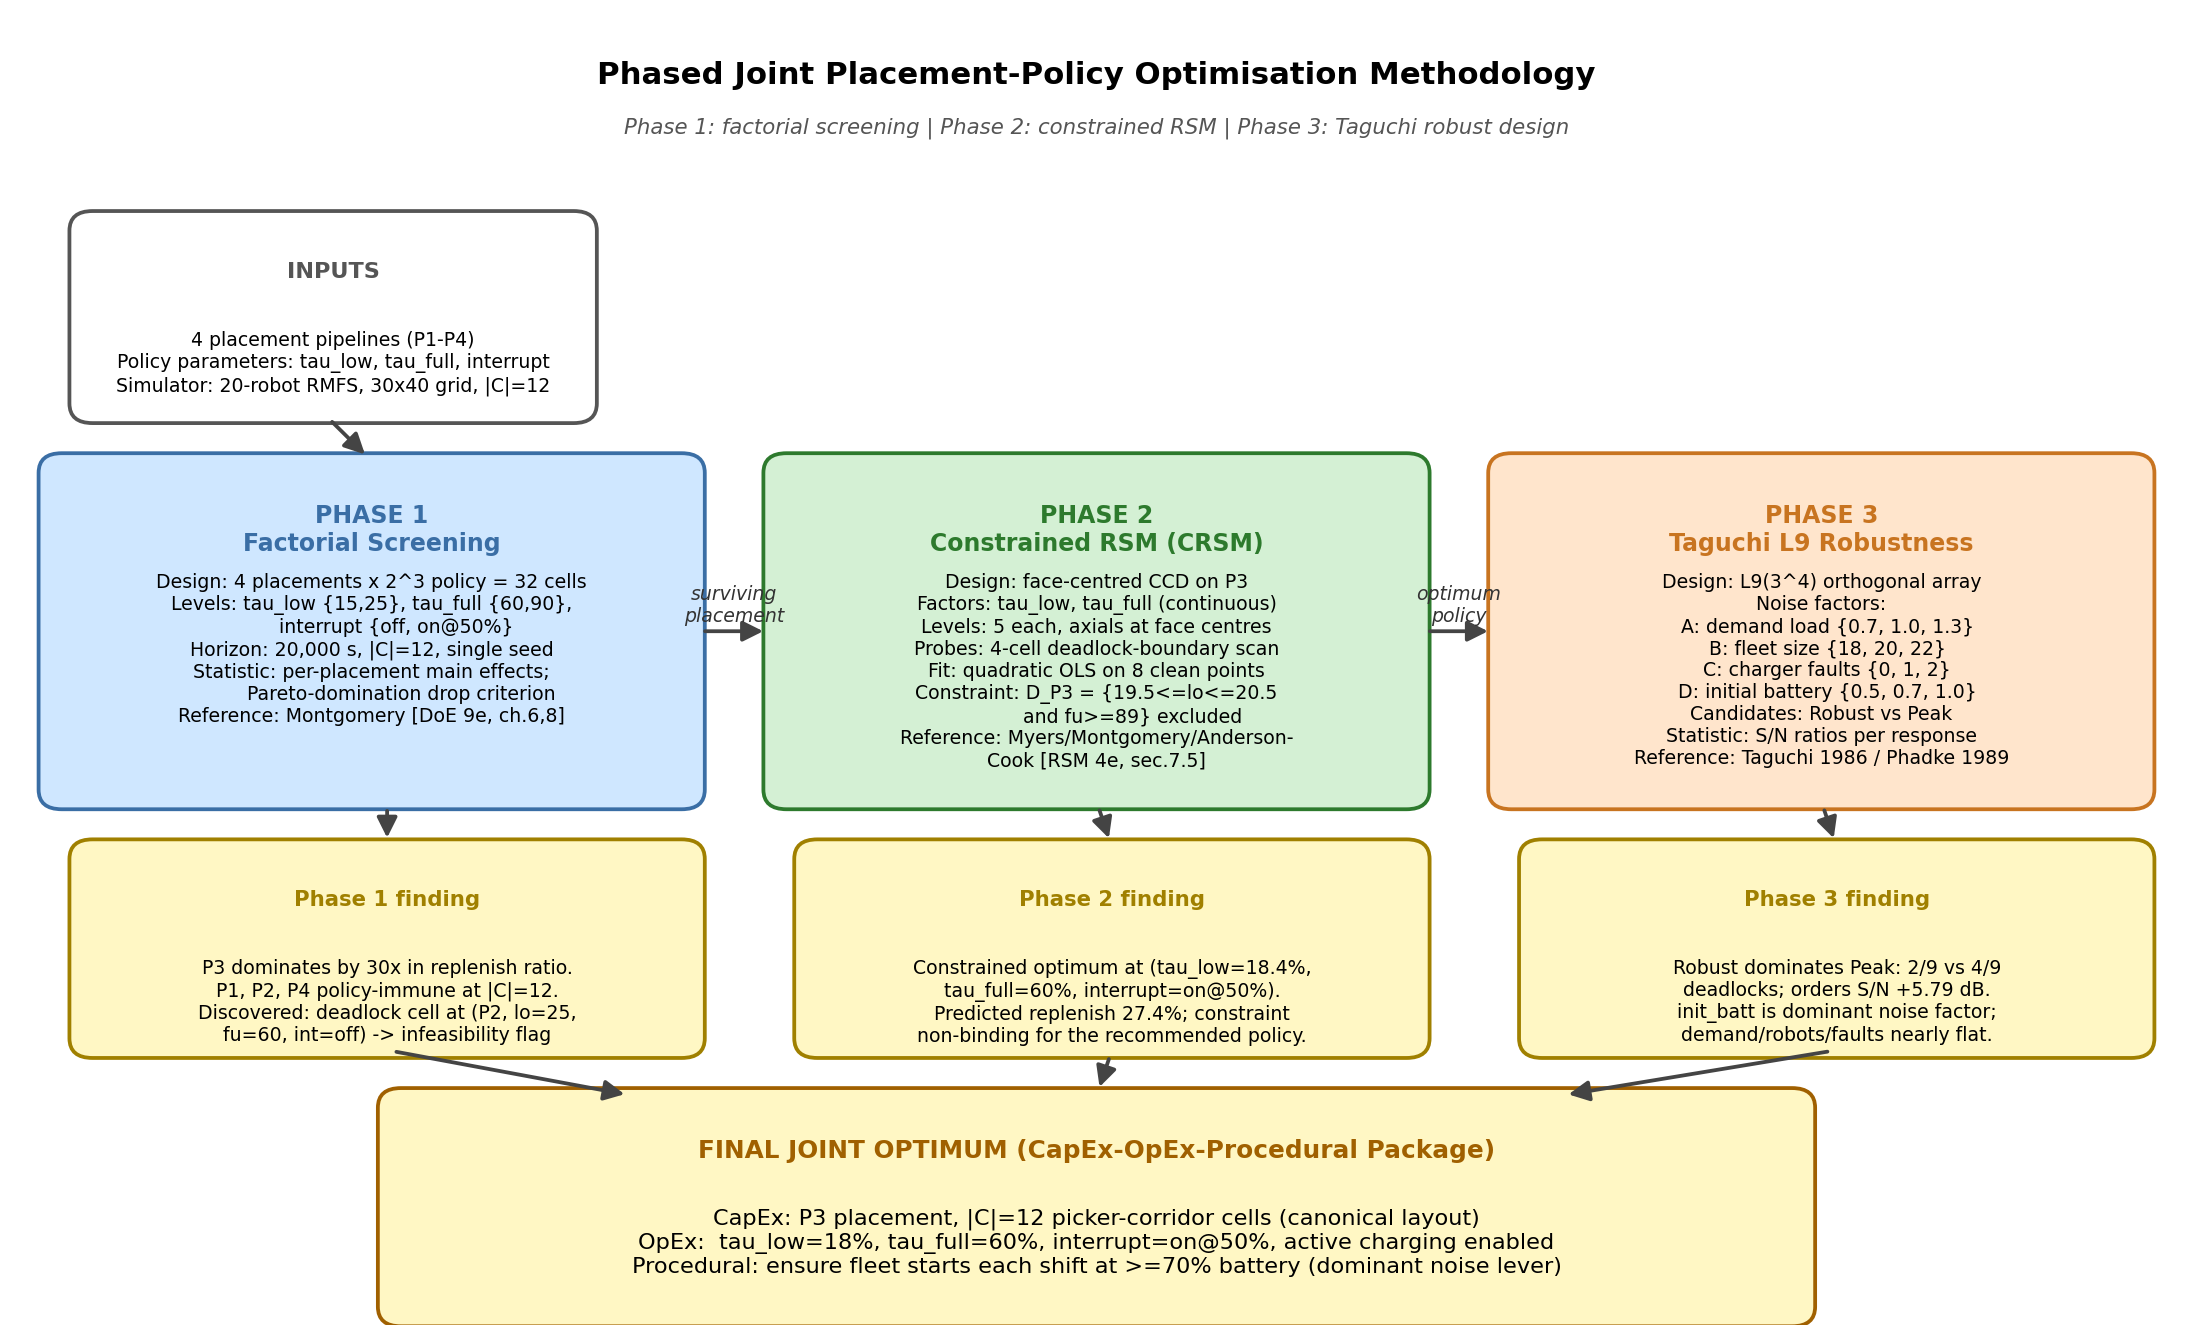
\includegraphics[width=\columnwidth]{methodology_flow.png}

    \column{0.45\textwidth}
    \footnotesize
    \textbf{Phase 1 --- Screening.} \\
    Four placements ($P_1$ Set-Cover, $P_2$ Affinity-Propagation, $P_3$ Picker-Station, $P_4$ Perimeter) at default policy. Long-horizon ($T = \SI{100000}{\second}$) + budget sweep.

    \vspace{0.3em}
    \textbf{Phase 2 --- Constrained RSM.} \\
    Face-centred CCD over policy thresholds on surviving placement. Discovered deadlock manifold treated as infeasibility constraint.

    \vspace{0.3em}
    \textbf{Phase 2b --- Cross-placement RSM.} \\
    21-cell design across all four placements + Michaelis--Menten saturation fit on $|C|$.

    \vspace{0.3em}
    \textbf{Phase 3 --- Taguchi $L_9$.} \\
    Four operational noise factors $\times$ S/N analysis comparing Phase-1 best vs Phase-2 RSM optimum.
  \end{columns}
\end{frame}

% ─────────────────────────────────────────────────────────────────────
\begin{frame}{Theory --- Design of Experiments and Response Surfaces}
  \footnotesize
  \textbf{Design of Experiments (DoE).}
  A statistical framework (Fisher, 1925; refined by Box \& Wilson, 1951) for systematically varying input factors and analysing their effect on a response variable, using as few experiments as possible while preserving statistical power.

  \vspace{0.4em}
  \textbf{Response Surface Methodology (RSM).}
  A second-stage DoE technique that fits a smooth polynomial model around an operating region:
  \[
    y = \beta_0 + \sum_i \beta_i x_i + \sum_i \beta_{ii} x_i^2 + \sum_{i<j} \beta_{ij} x_i x_j + \varepsilon
  \]
  The fitted surface enables analytical optimisation (gradient $= 0$, Hessian negative-definite) within the design region. Standard textbook reference: Myers, Montgomery \& Anderson-Cook (2016).

  \vspace{0.4em}
  \textbf{Central Composite Design (CCD).}
  The standard RSM design --- combines:
  \begin{itemize}
    \item $2^k$ factorial corners (estimate main effects + interactions)
    \item $2k$ axial points (estimate curvature)
    \item $n_c$ centre replicates (estimate pure error)
  \end{itemize}
  \textbf{Face-centred CCD} ($\alpha = 1$): axial points on the cube faces rather than outside. Chosen here because our factor bounds are operational limits, not just numerical; pushing axial points beyond them is physically meaningless.
\end{frame}

% ─────────────────────────────────────────────────────────────────────
\begin{frame}{Theory --- Why CCD, and Not Box-Behnken or Plackett-Burman?}
  \footnotesize
  \begin{tabular}{p{0.18\textwidth}p{0.32\textwidth}p{0.42\textwidth}}
    \toprule
    Design & Strength & Why not chosen here \\
    \midrule
    Plackett-Burman & Maximum screening power per run & Only main effects; no curvature, no interaction --- insufficient for an optimisation question. \\
    \addlinespace
    $2^k$ full factorial & Captures main effects + all interactions & Linear model only; cannot locate a smooth interior optimum. \\
    \addlinespace
    Box-Behnken & Avoids extreme-corner points & Doesn't sample the face/corner combinations where our deadlock manifolds live. Would have missed the constraint surface entirely. \\
    \addlinespace
    \textbf{Face-centred CCD} & Quadratic surface + corner coverage + boundary respect & \textbf{Chosen.} Reuses the Phase-1 factorial corners, samples the boundary where deadlock occurs, and supports analytical optimisation. \\
    \bottomrule
  \end{tabular}

  \vspace{0.5em}
  \textbf{Bottom line:} face-centred CCD is the only standard design that simultaneously supports quadratic curvature fitting, respects physical factor bounds, and reuses the screening corners we already ran in Phase 1.
\end{frame}

% ─────────────────────────────────────────────────────────────────────
\begin{frame}{Theory --- Constrained RSM and the Deadlock Manifold}
  \footnotesize
  \textbf{Standard RSM} assumes the response surface is smooth and differentiable across the design region. But in our simulator, certain $(\tau_\text{low}, \tau_\text{full})$ combinations trigger \textbf{deadlock} --- a discrete state in which robots block each other indefinitely. The response collapses to near-zero at these points.

  \vspace{0.4em}
  \textbf{Three options for handling discovered deadlock points:}
  \begin{enumerate}
    \item Drop them as outliers \\ $\Rightarrow$ statistically illegitimate; biases the fitted surface.
    \item Treat them as low-response observations \\ $\Rightarrow$ the quadratic fit becomes a worse model of the smooth region.
    \item \textbf{Treat them as an infeasibility region.} \\ $\Rightarrow$ fit the smooth model on the feasible subset; optimise subject to constraint $g(\boldsymbol{x}) \geq 0$, where $g$ separates safe from deadlock zones.
  \end{enumerate}

  \vspace{0.4em}
  \textbf{Constrained-RSM formulation (Myers, Montgomery \& Anderson-Cook, 2016):}
  \[
    \max_{\boldsymbol{x} \in \mathcal{D}}\; \hat{y}(\boldsymbol{x}) \quad \text{s.t.}\quad g(\boldsymbol{x}) \geq 0
  \]
  \textbf{Methodological contribution:} the constraint surface $g(\boldsymbol{x}) = 0$ \emph{is itself a research finding} --- it characterises the deadlock manifold rather than hiding it.
\end{frame}

% ─────────────────────────────────────────────────────────────────────
\begin{frame}{Theory --- Taguchi Robust Parameter Design}
  \footnotesize
  \textbf{Core idea (Taguchi, 1986):}
  A design is \emph{robust} if its performance is insensitive to uncontrollable noise factors. Optimising for robustness $\neq$ optimising for mean performance --- and the two can disagree.

  \vspace{0.4em}
  \textbf{Orthogonal arrays} (e.g.\ $L_9, L_{18}, L_{27}$) sample noise-factor combinations in a balanced way, allowing the noise envelope to be characterised in few runs. The $L_9(3^4)$ design probes four 3-level factors in only 9 runs (full factorial would need $3^4 = 81$).

  \vspace{0.4em}
  \textbf{Signal-to-Noise (S/N) ratios} convert mean and variance into a single optimisation target:
  \begin{align*}
    \text{Larger-the-better (LTB):} &\quad \eta_\text{LTB} = -10 \log_{10}\!\Big( \tfrac{1}{n} \textstyle\sum_i 1/y_i^2 \Big) \\
    \text{Smaller-the-better (STB):} &\quad \eta_\text{STB} = -10 \log_{10}\!\Big( \tfrac{1}{n} \textstyle\sum_i y_i^2 \Big)
  \end{align*}

  \vspace{0.3em}
  In our Phase 3: $y = $ orders completed (LTB), $y = $ energy per order (STB). Higher S/N is always better.

  \vspace{0.3em}
  \textbf{Our four noise factors:} demand load, fleet size, charger faults, initial battery state.
\end{frame}

% ─────────────────────────────────────────────────────────────────────
\begin{frame}{The Four Placement Algorithms}
  \footnotesize
  \begin{tabular}{p{0.13\textwidth}p{0.32\textwidth}p{0.42\textwidth}}
    \toprule
    Pipeline & Algorithm & Logic \\
    \midrule
    $P_1$ & \textbf{Set Cover Approximation} (greedy) & Classic NP-hard set-cover problem; covers high-traffic cells within radius $\rho$. Spreads chargers across the warehouse. \\
    \addlinespace
    $P_2$ & \textbf{Affinity Propagation} (Frey \& Dueck, 2007) & Message-passing clustering of high-traffic cells into exemplars. Self-determining number of clusters. \\
    \addlinespace
    $P_3$ & \textbf{Picker-Station Opportunistic} & Placement aligned to picker-station corridors. Robots charge during natural dwell time at stations $\Rightarrow$ no active charge trips. \\
    \addlinespace
    $P_4$ & \textbf{Perimeter Isolation} & Charger row on warehouse perimeter near replenishment stations. Acts as a control. \\
    \bottomrule
  \end{tabular}

  \vspace{0.5em}
  \textbf{Two design philosophies:} $P_1, P_2, P_4$ \emph{decouple} charging from the work flow (robots must leave their task to charge). $P_3$ \emph{couples} charging to the work flow (charging happens passively while the robot is already at a station). The performance gap between these philosophies is what Phase 1 quantifies.
\end{frame}

% ─────────────────────────────────────────────────────────────────────
\begin{frame}{Energy Model --- The Two-Channel Architecture}
  \footnotesize
  Battery drain is split into two physically independent channels:

  \vspace{0.4em}
  \textbf{Electronics channel} (mass-independent, constant 90 J/s):
  \[
    E_\text{idle}^{(\Delta t)} = P_\text{drain} \cdot \Delta t
  \]
  CPU, sensors, radio, lights. Active whenever not charging, regardless of payload.

  \vspace{0.4em}
  \textbf{Mechanical channel} (mass-scaled, motion-only):
  \begin{align*}
    E_\text{const} &= (m + m_L)\, g\mu\, v\, \Delta t \qquad\text{(rolling friction)} \\
    E_\text{accel} &= (m + m_L)\,(a\, k_\text{ir} + g\mu)\, v\, \Delta t \\
    E_\text{rot}   &= \tfrac{1}{6}(m+m_L)(L^2+W^2) \tfrac{\theta^2}{\tau_\text{rot}^2} + (m+m_L)g\mu r \theta \\
    E_\text{lift}  &= m_L \cdot g \cdot h_\text{lift}
  \end{align*}

  \vspace{0.3em}
  \textbf{Why the split matters:} a heavier robot standing still costs the same as an empty one (electronics-only). The cost of carrying a pod is paid only while the wheels are turning.

  \vspace{0.3em}
  \textbf{Battery spec (commercial AGV):} $E_\text{cap} = 1.8$\,kWh = 6.48\,MJ; $P_\text{charge} = $ 397.6\,W (= 28\,A $\times$ 14.2\,V); 5\,\%/hr idle drain $\Rightarrow$ 90\,J/s.
\end{frame}

% ─────────────────────────────────────────────────────────────────────
\begin{frame}{Phase 1 --- Placement Dominates Budget by an Order of Magnitude}
  \begin{columns}[T]
    \column{0.55\textwidth}
    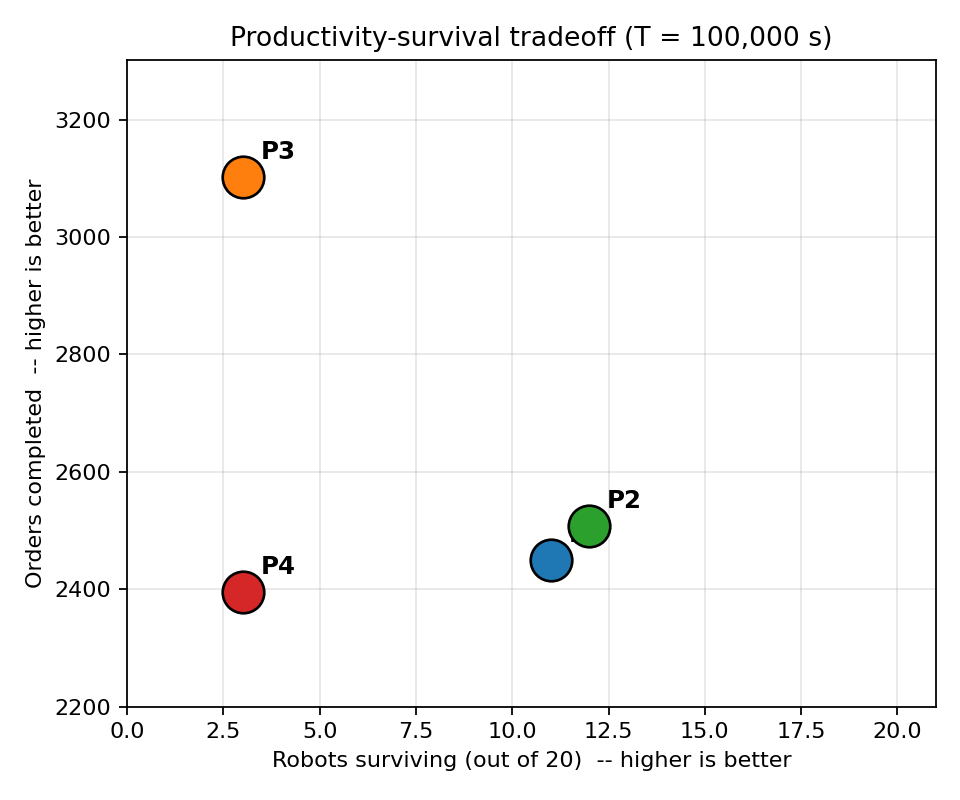
\includegraphics[width=\columnwidth]{tradeoff.png}

    \column{0.45\textwidth}
    \footnotesize
    \textbf{Long-horizon result} ($T = \SI{100000}{\second}$, $|C| = 12$, $N_r = 20$).

    \begin{itemize}
      \item $P_3$ (Picker-Tier) completes the most orders but loses fleet integrity.
      \item $P_2$ (Affinity Propagation) preserves fleet but completes fewer orders.
      \item $P_1$ sits between them.
      \item $P_4$ (Perimeter) is Pareto-dominated.
      \item \textbf{No placement at $|C|=12$ is operationally sustainable under default policy.}
    \end{itemize}

    \vspace{0.4em}
    \textbf{Replenish ratio gap:} $P_3$ achieves $\sim 30\times$ the replenishment-vs-consumption ratio of $P_1/P_2/P_4$.
  \end{columns}
\end{frame}

% ─────────────────────────────────────────────────────────────────────
\begin{frame}{Phase 1 --- Charger Budget Sweep Reveals $P_3$ Saturation}
  \begin{columns}[T]
    \column{0.6\textwidth}
    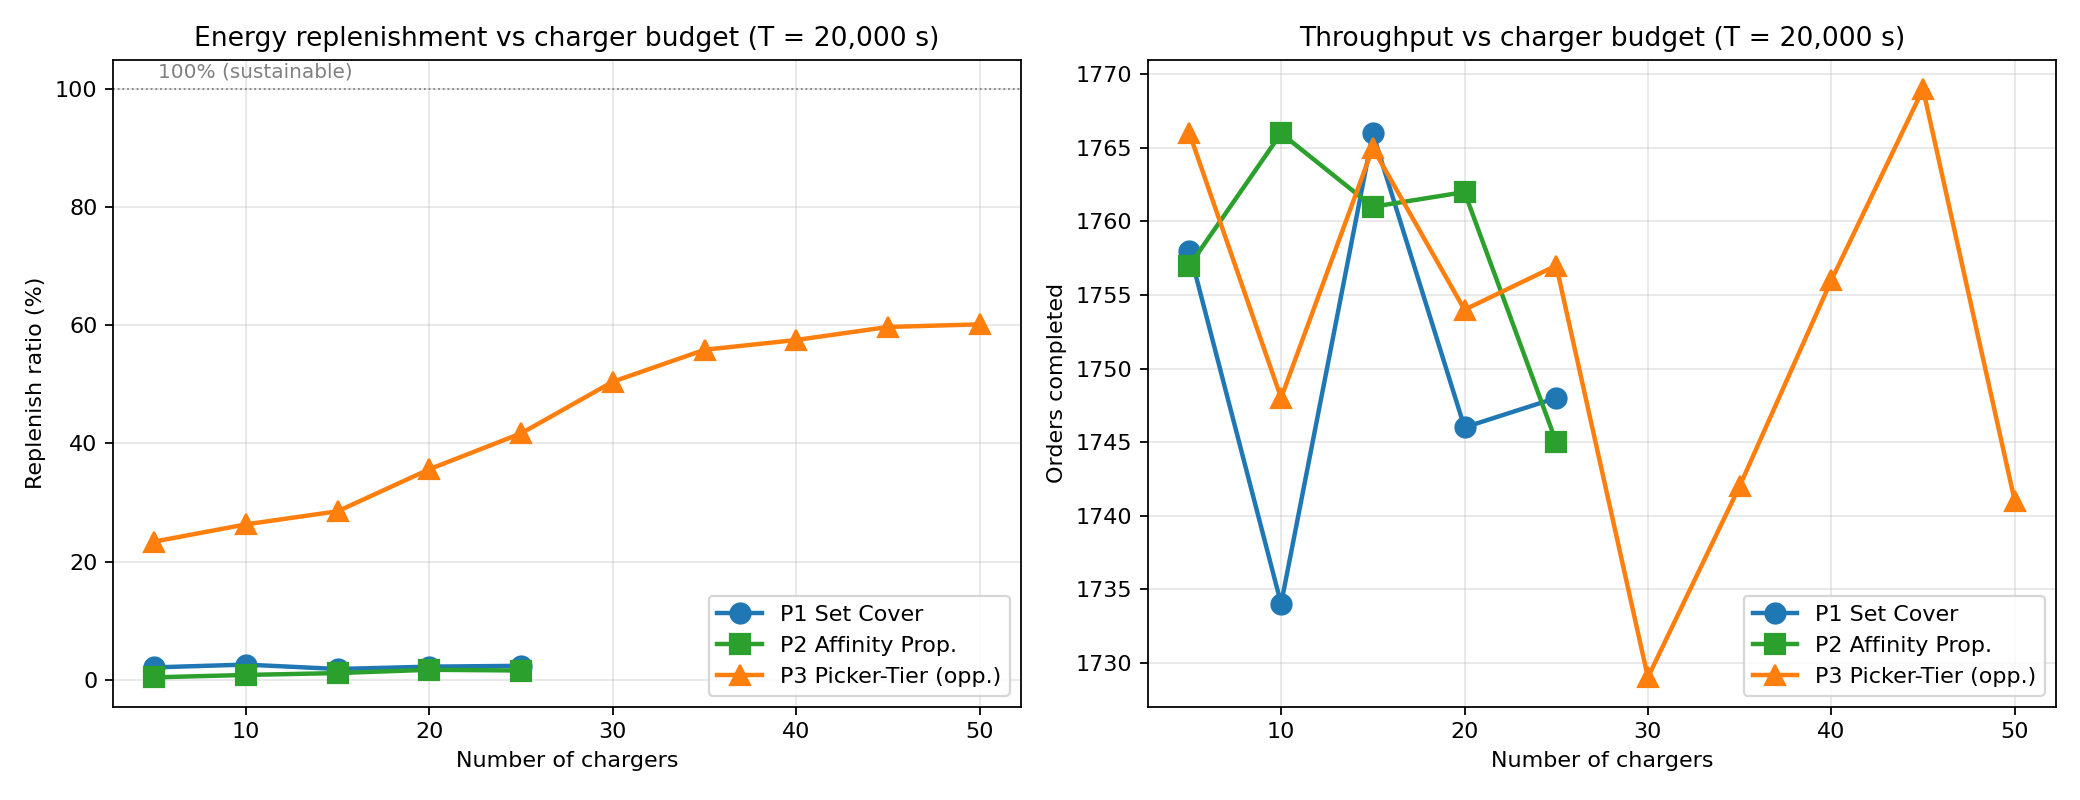
\includegraphics[width=\columnwidth]{combined_sweep.png}

    \column{0.4\textwidth}
    \footnotesize
    \textbf{Budget sweep} ($T = \SI{20000}{\second}$).

    \begin{itemize}
      \item $P_1, P_2$ essentially flat across budgets --- adding chargers does not help.
      \item $P_3$ climbs from 23\,\% $\to$ 60\,\% at $|C| = 50$.
      \item Marginal return drops sharply beyond $|C| = 35$.
      \item Saturation of the picker-tier heuristic.
    \end{itemize}

    \vspace{0.4em}
    \textbf{Cross-pipeline pattern:} placement geometry dominates. The threshold-policy lever exists but is an order of magnitude smaller than the placement lever.
  \end{columns}
\end{frame}

% ─────────────────────────────────────────────────────────────────────
\begin{frame}{Phase 1 --- Three Deadlock Mechanisms Observed}
  \begin{columns}[T]
    \column{0.55\textwidth}
    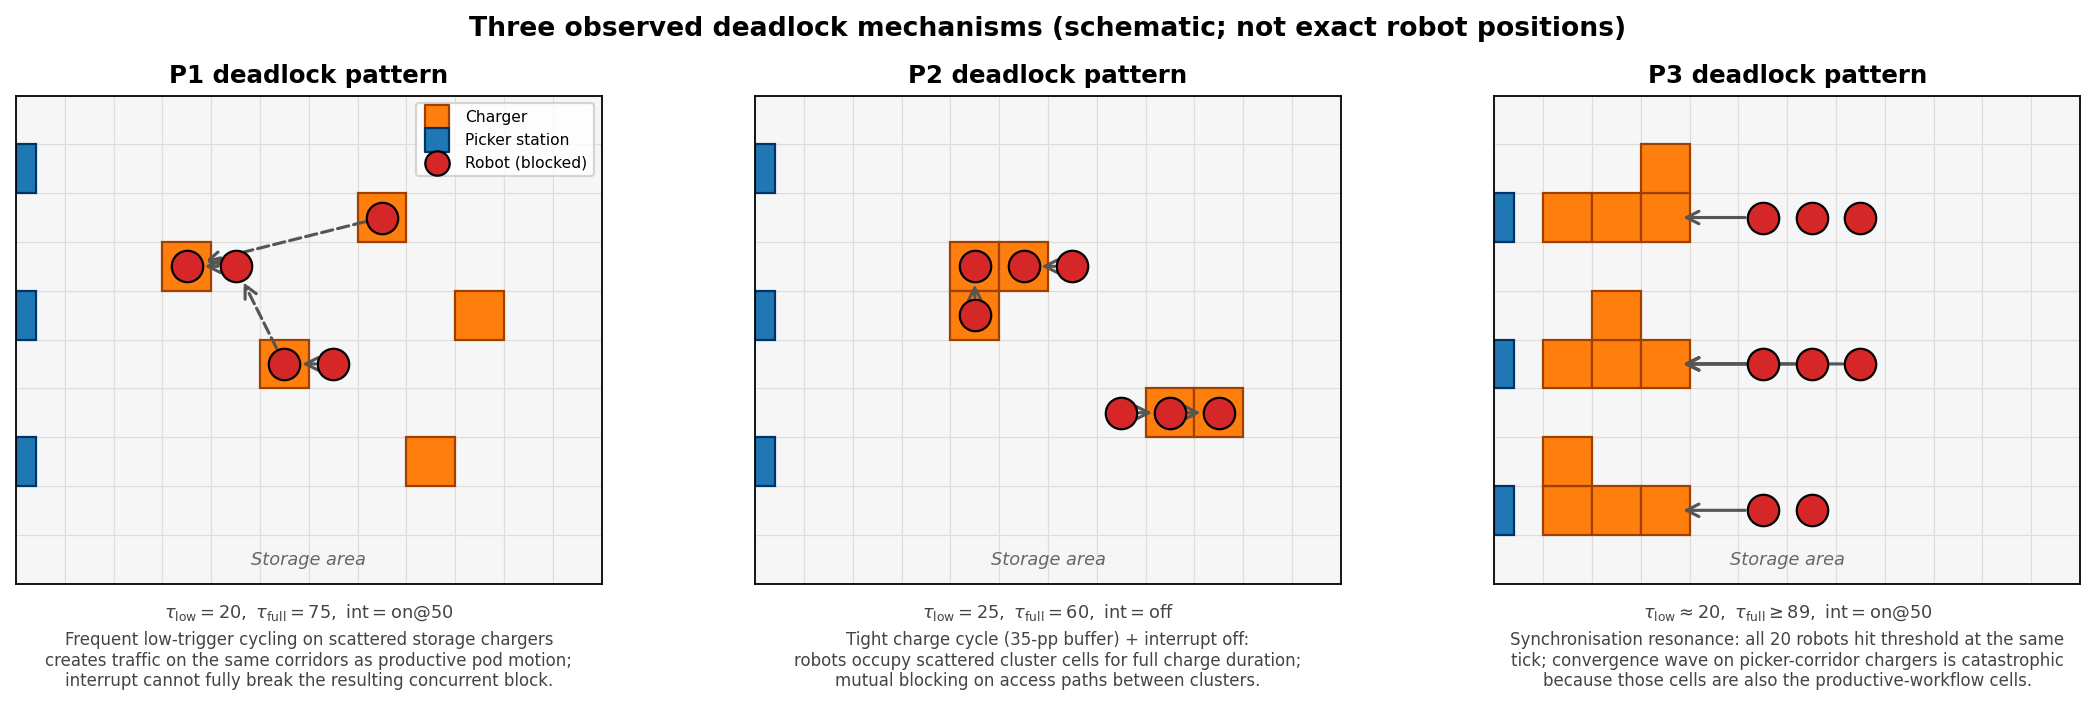
\includegraphics[width=\columnwidth]{deadlock_schematic.png}

    \column{0.45\textwidth}
    \footnotesize
    \textbf{Three deadlock failure modes observed in the run logs:}

    \begin{enumerate}
      \item \emph{$P_2$ contention wave:} aggressive trigger ($\tau_\text{low} = 25$, no interrupt) sends too many robots to charge at once.
      \item \emph{$P_3$ resonance:} interrupt at 50\,\% releases robots in synchronised waves that re-collide at picker stations.
      \item \emph{$P_1$ corridor block:} chargers placed in transit aisles create chokepoints when fleet is depleted.
    \end{enumerate}

    \vspace{0.3em}
    These three patterns motivated the Phase 2 constrained-RSM treatment.
  \end{columns}
\end{frame}

% ─────────────────────────────────────────────────────────────────────
\begin{frame}{Phase 2 --- Constrained RSM Identifies a Deadlock Manifold}
  \begin{columns}[T]
    \column{0.55\textwidth}
    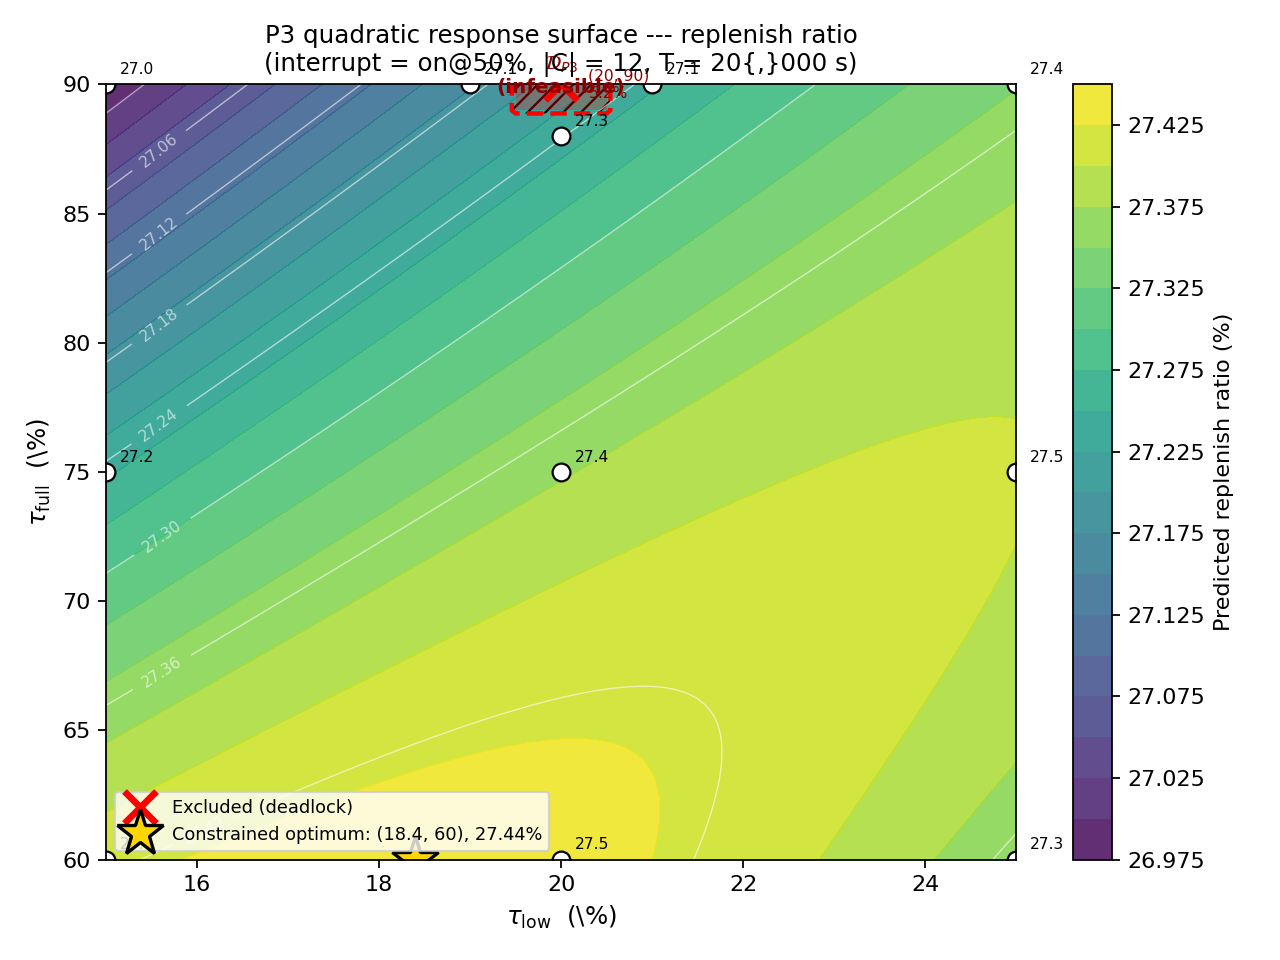
\includegraphics[width=\columnwidth]{phase2_rsm_surface.png}

    \column{0.45\textwidth}
    \footnotesize
    \textbf{Fitted quadratic surface ($P_3$ replenish ratio).}

    \begin{itemize}
      \item Thin deadlock zone discovered at $\tau_\text{low} \approx 20\,\%$, $\tau_\text{full} \geq 89\,\%$.
      \item Treated as infeasibility constraint --- not missing data.
      \item \textbf{Constrained optimum:}\\
        $\tau_\text{low} = 18\,\%$,\\
        $\tau_\text{full} = 60\,\%$,\\
        interrupt on @ 50\,\%.
    \end{itemize}

    \vspace{0.3em}
    \textbf{Phase 2b saturation fit:} Michaelis--Menten on $|C|/N_r$ shows $P_3$'s knee at $|C|/N_r \approx 0.5$ --- justifies $|C| = 12$ as the CapEx anchor.
  \end{columns}
\end{frame}

% ─────────────────────────────────────────────────────────────────────
\begin{frame}{Phase 3 --- Robust Beats Peak on Mean \emph{and} Robustness}
  \begin{columns}[T]
    \column{0.5\textwidth}
    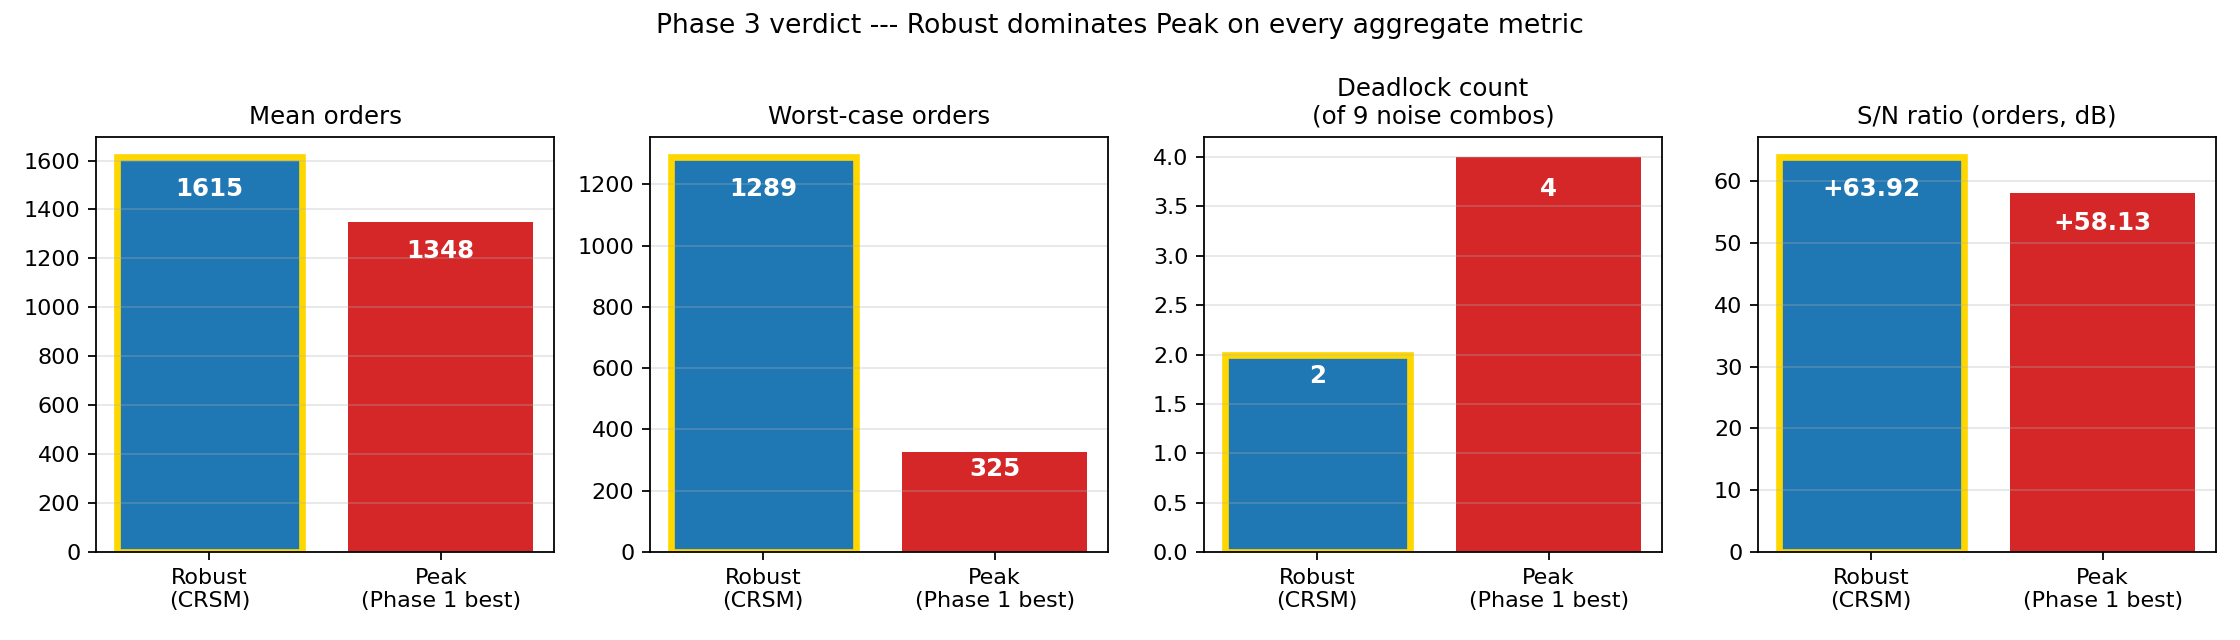
\includegraphics[width=\columnwidth]{phase3_robust_vs_peak.png}

    \column{0.5\textwidth}
    \scriptsize
    \begin{tabular}{lrr}
      \toprule
      Metric & Peak & Robust \\
      \midrule
      Mean orders ($L_9$)  & 1{,}348.1 & \textbf{1{,}614.7} \\
      Deadlocked cells     & 4/9       & \textbf{2/9} \\
      Orders S/N (dB)      & ---       & \textbf{+5.79} \\
      $\eta_E$ (kJ/order)  & 48.8      & \textbf{44.4} \\
      \bottomrule
    \end{tabular}

    \vspace{0.5em}
    \footnotesize
    \textbf{Candidates compared:}
    \begin{itemize}
      \item \emph{Peak:} Phase-1 best corner (interrupt off).
      \item \emph{Robust:} Phase-2 constrained-RSM optimum.
    \end{itemize}

    \vspace{0.3em}
    Robust dominates across \emph{every} aggregate metric --- mean, robustness, deadlock, and energy cost per order.
  \end{columns}
\end{frame}

% ─────────────────────────────────────────────────────────────────────
\begin{frame}{Phase 3 --- Initial Battery State is the Dominant Noise Lever}
  \begin{columns}[T]
    \column{0.6\textwidth}
    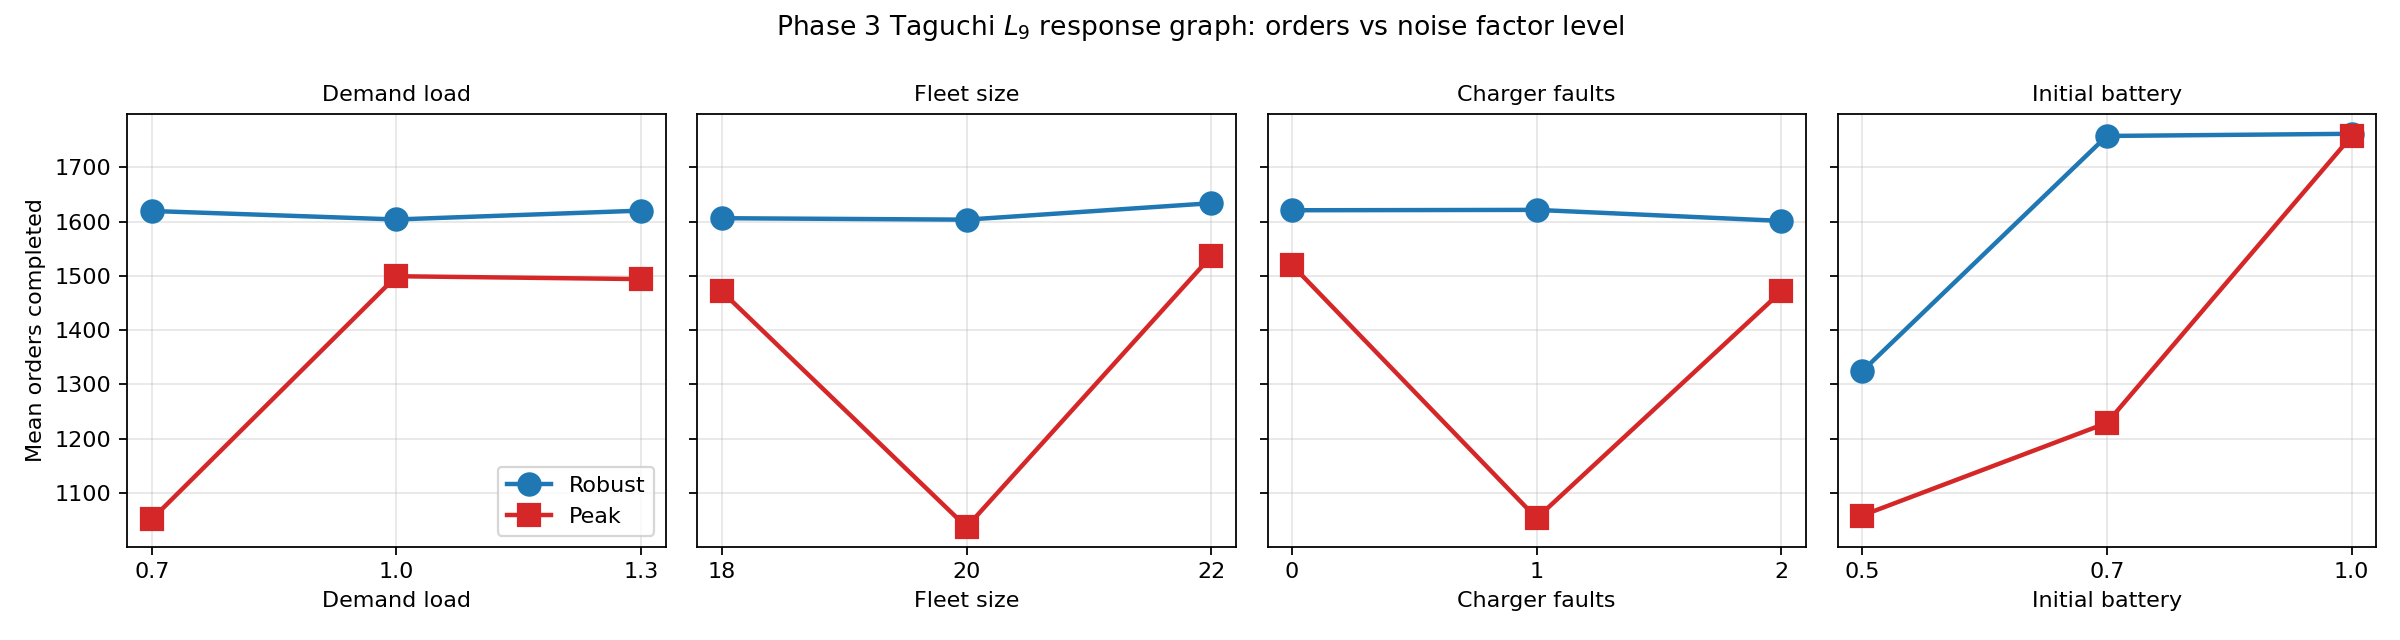
\includegraphics[width=\columnwidth]{phase3_taguchi_response.png}

    \column{0.4\textwidth}
    \footnotesize
    \textbf{Taguchi response graph:} order count vs level for each noise factor.

    \begin{itemize}
      \item \emph{Initial battery:} largest swing across levels.
      \item Demand swing $\pm 30\,\%$: absorbed.
      \item One to two charger faults: absorbed.
      \item Fleet attrition $\pm 2$: absorbed.
    \end{itemize}

    \vspace{0.4em}
    \textbf{Counter-intuitive insight:} the controllable lever is \emph{not} demand or fleet size --- it is start-of-shift battery state. The procedural fix is a shift-handover protocol, not a demand-forecasting investment.
  \end{columns}
\end{frame}

% ─────────────────────────────────────────────────────────────────────
\begin{frame}{Decision-Grade Output --- CapEx, OpEx, Procedural}
  \footnotesize
  \begin{tabular}{p{0.18\textwidth}p{0.34\textwidth}p{0.42\textwidth}}
    \toprule
    \textbf{Tier} & \textbf{Recommendation} & \textbf{Justification} \\
    \midrule
    CapEx & $P_3$ placement; $|C| = 12$ chargers in picker corridor & $30\times$ replenish margin over $P_1/P_2/P_4$; saturation knee below $|C| = N_r$ \\
    \addlinespace
    OpEx & $\tau_\text{low} = 18\,\%$, $\tau_\text{full} = 60\,\%$, interrupt on @ 50\,\% & Phase-2 constrained-RSM optimum; confirmed as robust optimum in Phase 3 \\
    \addlinespace
    Procedural & Ensure $\geq 70\,\%$ start-of-shift battery & Phase-3 dominant noise factor; $50\,\%$ start state risks deadlock \\
    \bottomrule
  \end{tabular}

  \vspace{0.8em}
  Each tier is traceable to a specific experimental phase, and each decision is defended by the corresponding statistical machinery: response surfaces (Phase 2), signal-to-noise ratios (Phase 3), deadlock-manifold characterisation (Phase 1--2).
\end{frame}

% ─────────────────────────────────────────────────────────────────────
\begin{frame}{Financial Projection --- Solusi Memiliki Fundamental Finansial yang Kokoh}
  \footnotesize
  \begin{columns}[T]
    % ── Estimasi Parameter ────────────────────────────────────────────
    \column{0.30\textwidth}
    \begin{block}{\color{boxblue}\textbf{Estimasi Parameter}}
      \scriptsize
      \textbf{Operating Profile}\\ 2 shifts $\times$ 4{,}800 hr/yr \\[2pt]
      \textbf{Electricity (Taipower)}\\ NT\$3.50/kWh \\[2pt]
      \textbf{Margin per Pick}\\ NT\$15/order (grocery) \\[2pt]
      \textbf{Charger Cost}\\ NT\$155k + NT\$46.5k install \\[2pt]
      \textbf{Relocation}\\ NT\$37.2k per unit \\[2pt]
      \textbf{Tax / WACC}\\ 20\% / 10\% \\[2pt]
      \textbf{Battery Life $\uparrow$}\\ +30\% at $\tau_\text{full}{=}60\%$ \\[2pt]
      \textbf{Currency}\\ NT\$31 = USD\$1
    \end{block}

    % ── Cash flow chart ──────────────────────────────────────────────
    \column{0.40\textwidth}
    \centering
    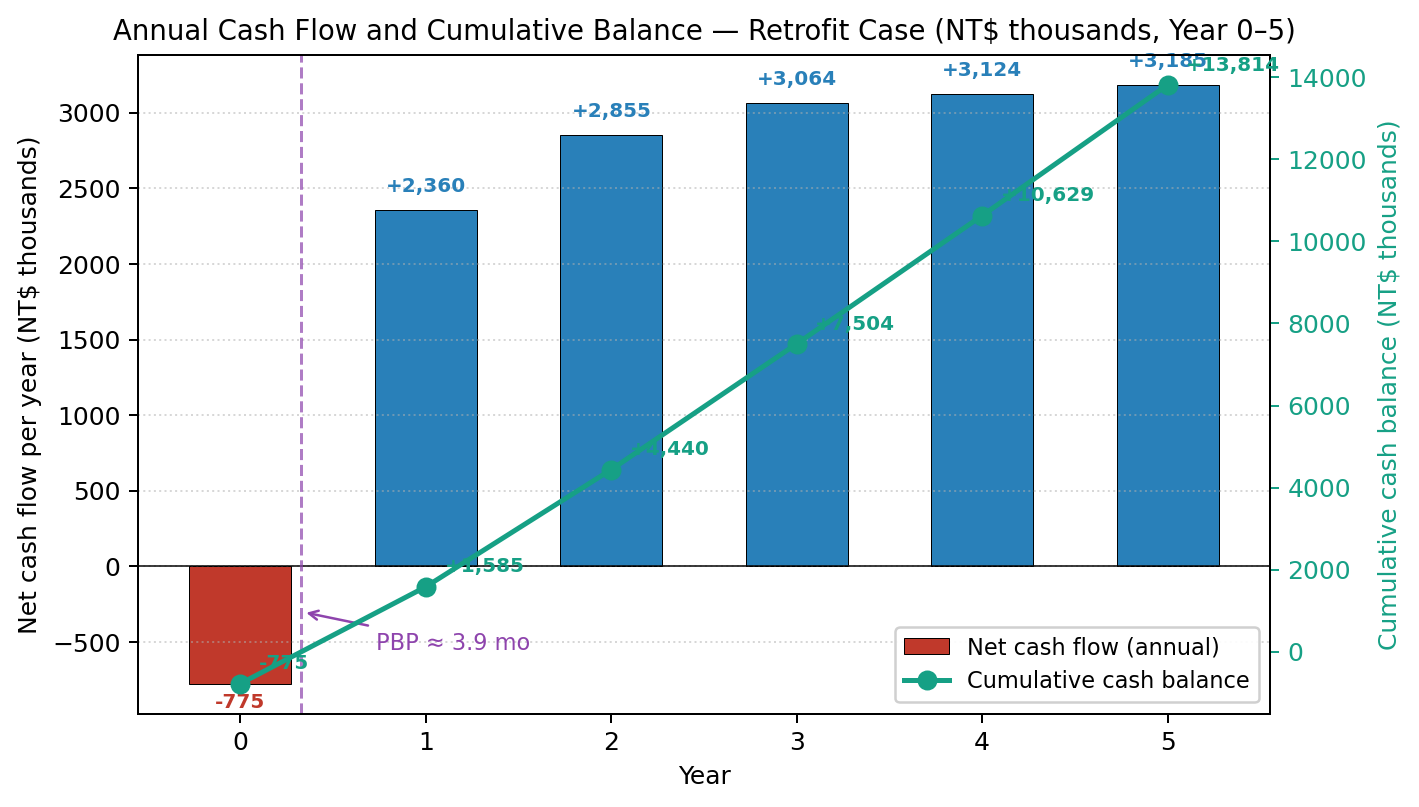
\includegraphics[width=\columnwidth]{financial_cashflow_bars.png}\\
    \tiny Net Cash Flow (bars) \& Cumulative Balance (line), Retrofit case

    % ── Proyeksi Finansial highlights ────────────────────────────────
    \column{0.28\textwidth}
    \begin{block}{\color{boxblue}\textbf{Proyeksi Finansial}}
      \scriptsize
      \textbf{\Large 3.9 mo}\\ Payback Period \\[3pt]
      \textbf{\Large 304\%}\\ 5-yr IRR \\[3pt]
      \textbf{\Large NT\$10.1 M}\\ 5-yr NPV @ 10\% \\[3pt]
      \textbf{\Large NT\$2.9--4.0 M}\\ Annual revenue gain \\[3pt]
      \textbf{\Large 204\%}\\ Year-1 ROI
    \end{block}

    \begin{block}{\color{boxgreen}\textbf{Verdict}}
      \scriptsize
      Tren positif yang signifikan menandakan solusi \textbf{layak dijalankan.}
    \end{block}
  \end{columns}
\end{frame}

% ─────────────────────────────────────────────────────────────────────
\begin{frame}{Financial Projection --- CapEx \& OpEx Breakdown}
  \footnotesize
  \begin{columns}[T]
    \column{0.5\textwidth}
    \textbf{\color{boxblue} CapEx (Year 0 --- One-Time Investment)} \\
    \vspace{0.3em}
    \begin{tabular}{p{0.55\columnwidth}rr}
      \toprule
      Item & Qty & NT\$ (thousands) \\
      \midrule
      Industrial charger unit & 2 & 310.0 \\
      Installation (anchor + wiring) & 2 & 93.0 \\
      Relocation of existing chargers & 10 & 372.0 \\
      \midrule
      \textbf{Total CapEx} & & \textbf{775.0} \\
      \bottomrule
    \end{tabular}

    \vspace{0.6em}
    \textbf{\color{boxblue} Depreciation (5-yr straight-line)}
    \[
      D = \frac{\text{NT\$}775\text{k}}{5} = \text{NT\$}155\text{k/yr}
    \]
    Non-cash; reduces taxable income $\Rightarrow$ tax shield $D \cdot t = \text{NT\$}31\text{k/yr}$.

    \column{0.5\textwidth}
    \textbf{\color{boxgreen} OpEx Delta (Year 1, before ramp \& inflation)} \\
    \vspace{0.3em}
    \begin{tabular}{p{0.55\columnwidth}rr}
      \toprule
      Item & Type & NT\$/yr (thousands) \\
      \midrule
      Revenue gain (244{,}320 picks $\times$ NT\$15) & + & 3{,}664.8 \\
      Energy saving (2{,}630 kWh $\times$ NT\$3.50) & + & 9.2 \\
      Battery longevity \emph{(excluded --- not modelled)} & --- & 0.0 \\
      Maintenance (7\% $\times$ new CapEx NT\$403k) & $-$ & 28.2 \\
      \midrule
      \textbf{Pre-tax cash benefit (full-ramp)} & & \textbf{3{,}645.8} \\
      \bottomrule
    \end{tabular}

    \vspace{0.6em}
    \textbf{\color{boxgreen} Year-on-Year Dynamics}
    \begin{itemize}
      \item Ramp: 80\% / 95\% / 100\% / 100\% / 100\%
      \item Revenue inflation: +2\%/yr (CPI pass-through)
      \item Energy inflation: +3\%/yr (Taipower trend)
      \item Maintenance escalation: +5\%/yr
    \end{itemize}
  \end{columns}
\end{frame}

% ─────────────────────────────────────────────────────────────────────
\begin{frame}{Financial Projection --- 5-Year Cash Flow Projection}
  \scriptsize
  \begin{columns}[T]
    \column{0.65\textwidth}
    \textbf{\color{boxblue} Pre-Tax Income (NT\$ thousands)}\\
    \vspace{0.2em}
    \begin{tabular}{lrrrrr}
      \toprule
      Year & 1 & 2 & 3 & 4 & 5 \\
      \midrule
      Revenue gain   & 2{,}931.8 & 3{,}551.0 & 3{,}812.8 & 3{,}889.1 & 3{,}966.9 \\
      Energy save    & 7.4 & 9.0 & 9.8 & 10.1 & 10.4 \\
      Maintenance    & $-28.2$ & $-29.6$ & $-31.1$ & $-32.6$ & $-34.3$ \\
      \midrule
      \textbf{Pre-tax} & \textbf{2{,}911.0} & \textbf{3{,}530.4} & \textbf{3{,}791.5} & \textbf{3{,}866.6} & \textbf{3{,}943.0} \\
      \bottomrule
    \end{tabular}
    \tiny\emph{Battery longevity excluded --- degradation not modelled (Limitations).}

    \vspace{0.4em}
    \textbf{\color{boxgreen} Net Income \& After-Tax Cash Flow (NT\$ thousands)}\\
    \vspace{0.2em}
    \scriptsize
    \begin{tabular}{lrrrrr}
      \toprule
      Year & 1 & 2 & 3 & 4 & 5 \\
      \midrule
      Pre-tax        & 2{,}911.0 & 3{,}530.4 & 3{,}791.5 & 3{,}866.6 & 3{,}943.0 \\
      Depreciation   & $-155.0$  & $-155.0$  & $-155.0$  & $-155.0$  & $-155.0$ \\
      Taxable income & 2{,}756.0 & 3{,}375.4 & 3{,}636.5 & 3{,}711.6 & 3{,}788.0 \\
      Tax (20\%)     & $-551.2$  & $-675.1$  & $-727.3$  & $-742.3$  & $-757.6$ \\
      \midrule
      \textbf{ATCF}  & \textbf{2{,}359.8} & \textbf{2{,}855.3} & \textbf{3{,}064.2} & \textbf{3{,}124.3} & \textbf{3{,}185.4} \\
      \textbf{Cumul.}& \textbf{1{,}584.8} & \textbf{4{,}440.1} & \textbf{7{,}504.4} & \textbf{10{,}628.7} & \textbf{13{,}814.1} \\
      \bottomrule
    \end{tabular}

    \column{0.35\textwidth}
    \begin{block}{\color{boxpurple}\textbf{Perhitungan Proyeksi}}
      \tiny
      \textbf{Revenue}$_y = \Delta N \cdot m \cdot \rho_y \cdot (1{+}\iota_R)^{y-1}$\\[2pt]
      $\Delta N = 244{,}320$ picks/yr at full ramp\\[2pt]
      \textbf{Energy save}$_y = \Delta E \cdot p_e \cdot \rho_y \cdot (1{+}\iota_E)^{y-1}$\\[2pt]
      \textbf{Maintenance}$_y = -0.07 \cdot \text{CapEx}_\text{new} \cdot (1{+}\iota_M)^{y-1}$\\[3pt]
      \textbf{Pre-tax}$_y$ = sum of above\\[2pt]
      \textbf{Tax}$_y = -t \cdot (\text{Pre-tax}_y - D)$\\[2pt]
      \textbf{ATCF}$_y = \text{Pre-tax}_y + \text{Tax}_y$\\[3pt]
      \textbf{PBP} = interpolated zero-crossing of cumulative ATCF\\[2pt]
      \textbf{NPV}$_5 = -\text{CapEx} + \sum_{y=1}^{5} \frac{\text{ATCF}_y}{(1{+}r)^y}$\\[2pt]
      \textbf{IRR}: solve $\sum \frac{\text{ATCF}_y}{(1{+}\text{IRR})^y} = \text{CapEx}$\\[3pt]
      \emph{Battery saving deliberately excluded.}
    \end{block}

    \begin{block}{\color{boxblue}\textbf{Headline}}
      \scriptsize
      PBP = 3.9 months \\
      NPV$_5$ = NT\$10{,}144k \\
      IRR = 304\% \\
      Year-1 ROI = 204\%
    \end{block}
  \end{columns}
\end{frame}

% ─────────────────────────────────────────────────────────────────────
\begin{frame}{The RL Extension --- A Documented Negative Result}
  \footnotesize
  \textbf{Why we tried RL.} The literature (Bischoff et al.\ 2025, Singh et al.\ 2024) reports that learned policies can refine threshold-based heuristics by a few percent. We wanted to test whether the same held on our environment.

  \vspace{0.4em}
  \textbf{Setup.} MaskablePPO (Proximal Policy Optimization with action masking; sb3-contrib). Per-AMR-per-event decisions; 9 discrete charge targets; 15-dim observation. Four configurations exercised on $P_1$.

  \vspace{0.4em}
  \textbf{Outcome.} All four runs collapsed within 4--8 PPO iterations: policy entropy $\to 0$, action mass concentrated on action 0 (``no charge''), mean reward decayed monotonically as the all-action-0 policy drove robots into depletion.

  \vspace{0.4em}
  \textbf{Three structural root causes:}
  \begin{enumerate}
    \item \emph{Action-mask asymmetry.} Action 0 is always legal; charge actions require $t > b$.
    \item \emph{Reward myopia.} Per-decision reward $\Delta\text{orders}$ pays off immediately; battery-depletion penalty fires $\sim 1000$ ticks later --- beyond PPO's $\gamma = 0.99$ effective horizon ($\sim 100$ steps).
    \item \emph{Decision-granularity asymmetry.} Action 0 returns the agent to the next event quickly; charge actions silence the focal robot for many ticks $\Rightarrow$ sparser reward signal.
  \end{enumerate}

  \vspace{0.3em}
  \textbf{Implication:} the collapse \emph{strengthens} the methodological choice. Fixing it requires re-engineering the env in ways that decouple RL from the heuristic baseline it would refine --- partly defeating the original motivation.
\end{frame}

% ─────────────────────────────────────────────────────────────────────
\begin{frame}{Limitations and Future Work}
  \footnotesize
  \textbf{Limitations of the present study:}
  \begin{itemize}
    \item Single-seed deterministic protocol (no pure-error variance estimate from replicates).
    \item Policy axis restricted to the three-knob threshold class ($\tau_\text{low}, \tau_\text{full}$, interrupt).
    \item Deadlock manifolds characterised within the immediate neighbourhood of the design centre; wider sweeps may reveal additional infeasible regions.
    \item No regenerative braking, no charging curve, perfectly flat warehouse floor.
  \end{itemize}

  \vspace{0.5em}
  \textbf{Future work:}
  \begin{itemize}
    \item Multi-seed replication of Phase 2 and Phase 3 for pure-error variance estimation.
    \item Hybrid placements combining $P_3$'s dwell-alignment with $P_1/P_2$'s spatial spread.
    \item Capacity-vs-count comparison: raising $E_\text{cap}$ instead of $|C|$.
    \item Re-engineered RL environment (dense battery-cost shaping, null-action-free space, fleet-level decisions) to test whether a learned policy can break the depletion ceiling.
  \end{itemize}
\end{frame}

% ─────────────────────────────────────────────────────────────────────
\begin{frame}
  \begin{center}
    \vspace{1cm}
    {\Huge Thank You.}

    \vspace{1.2cm}
    {\Large Questions \& Discussion}

    \vspace{1cm}
    \footnotesize
    Salsa Zahrani \\
    Engineering Management, Institut Teknologi Bandung \\
    \texttt{nazzahraarezta@gmail.com}
  \end{center}
\end{frame}

\end{document}
